\documentclass{homework}

\newcommand{\hwname}{张学涵}
\newcommand{\hwemail}{xxhzhang@mail.ustc.edu.cn}
\newcommand{\hwtype}{作业}
\newcommand{\hwnum}{1}
\newcommand{\hwclass}{复变函数 B}
\newcommand{\hwlecture}{宁吴庆}
\newcommand{\hwsection}{}

\begin{document}
\maketitle

\question{1}
% \subquestion{1} \((3-\sqrt{3}i)(3+\sqrt{3}i)=3^2+\sqrt{3}^2=12\)
\subquestion{2}
\(\begin{aligned}[t](x-i\sqrt{y})(-x-2i\sqrt{y})&=-x^2-2ix\sqrt{y}+ix\sqrt{y}-2y\\&=-x^2-2y-ix\sqrt{y}.\end{aligned}\)

\subquestion{3}
\(\frac{3-4i}{4+3i}=\frac{(3-4i)(4-3i)}{25}=\frac{12-12-25i}{25}=-i.\)

% \subquestion{4} \(\frac{5i}{\sqrt{2}-\sqrt{3}i}=\frac{5i(\sqrt{2}+\sqrt{3}i)}{5}=-\sqrt{3}+\sqrt{2}i\)

\question{2}
\subquestion{3}
\(\begin{aligned}[t]z&=\frac{\sqrt{13}}{2}e^{i(-\pi+\arctan{2}\sqrt{3})}\\&=\frac{\sqrt{13}}{2}(\cos(-\pi+\arctan{2}\sqrt{3})+i\sin(-\pi+\arctan{2}\sqrt{3})),\end{aligned}\)

\(\mathrm{Arg} z=\arg z+2k\pi=-\pi+\arctan{2}\sqrt{3}+2k\pi, k\in\mathbb{Z}\).

\subquestion{4}
若 \(\theta=2k\pi, k\in\mathbb{Z}\), 则 \(z=0\), 辐角无意义.

否则设 \(\theta=2k\pi+\theta_0, \theta_0\in(0, 2\pi)\), 则

\(\begin{aligned}[t]z&=2\sin\frac{\theta_0}{2}e^{i(\frac{\pi-\theta_0}{2})}\\&=2\sin\frac{\theta_0}{2}(\cos\frac{\pi-\theta_0}{2}+i\sin\frac{\pi-\theta_0}{2}),\end{aligned}\)

\(\mathrm{Arg} z=\arg z+2k\pi=\frac{\pi-\theta_0}{2}+2k\pi, k\in\mathbb{Z}\).

\fbox{\parbox{\textwidth}{注释:\begin{enumerate}
  \item 很多人没有讨论 \(z\) 是否为 0.
  \item 如果不约束 \(\theta_0\in(0, 2\pi)\), 而是直接用 \(\theta\) 表示, 需要注意 \(\sqrt{2-2\cos{\theta}}=\sqrt{4\sin^2{\frac{\theta}{2}}}=2\lvert\sin\frac{\theta}{2}\rvert\).
\end{enumerate}}}

\question{3}
\subquestion{3}
\(\sqrt[3]{1+i}\begin{aligned}[t]&=\left(\sqrt{2}e^{i(\frac{\pi}{4}+2k\pi)}\right)^{\frac{1}{3}}\\&=\sqrt[6]{2}e^{i(\frac{\pi}{12}+\frac{2k\pi}{3})}, k=0,1,2.\end{aligned}\)

\question{4}
\subquestion{2}
\(\begin{aligned}[t]z&=\left(e^{i(-\frac{\pi}{2}+2k\pi)}\right)^{\frac{1}{3}}\\&=e^{i(-\frac{\pi}{6}+\frac{2k\pi}{3})}, k=0,1,2.\end{aligned}\)

\subquestion{3}
\(\begin{aligned}[t]z&=\left(e^{i\pi+2k\pi}\right)^{\frac{1}{4}}\\&=e^{i(\frac{\pi}{4}+\frac{k\pi}{2})}, k=0,1,2,3.\end{aligned}\)

\question{6}
两边平方得 \(x^2-y^2+2ixy=a+ib\), 故
\(\begin{cases}x^2-y^2=a;\\2xy=b.\end{cases}\)

\(2xy=b \Rightarrow 4x^2y^2=b^2 \Rightarrow 4x^2(x^2-a)=b^2\),
解得 $\begin{cases}x^2=\frac{a+\sqrt{a^2+b^2}}{2};\\y^2=\frac{-a+\sqrt{a^2+b^2}}{2}.\end{cases}$

再次注意到 \(2xy=b\), 所以 \(\begin{cases}x=\pm\sqrt{\frac{a+\sqrt{a^2+b^2}}{2}};\\y=\pm\sqrt{\frac{-a+\sqrt{a^2+b^2}}{2}}.\end{cases}\)

其中 \(b>0\) 时 \(x,y\) 同号, \(b<0\) 时 \(x,y\) 异号, \(b=0\) 时 \(y=0\).

\question{7}
令 \(z=\cos\theta+i\sin\theta\), 则
\[\sum_{k=1}^nz^k=\sum_{k=1}^n\cos{k\theta}+i\sum_{k=1}^n\sin{k\theta}.\]
只需求
\[\sum_{k=1}^nz^k=\begin{cases}
z\frac{z^n-1}{z-1} & \text{ if } z \neq 1;\\
n & \text{ if } z = 1.
\end{cases}\]
的实部和虚部即可. 如 \(z\neq1\),
\begin{align*}
  z-1&=(\cos\theta-1)+i\sin\theta\\
  &=-2\sin^2\frac{\theta}{2}+2i\sin\frac{\theta}{2}\cos\frac{\theta}{2}\\
  &=-2\sin\frac{\theta}{2}\left(\cos(\frac{\pi}{2}-\frac{\theta}{2})-i\sin(\frac{\pi}{2}-\frac{\theta}{2})\right)\\
  &=-2\sin\frac{\theta}{2}e^{i(\frac{\theta}{2}-\frac{\pi}{2})}.
\end{align*}
同理,
\[z^n-1=-2\sin\frac{n\theta}{2}e^{i(\frac{n\theta}{2}-\frac{\pi}{2})}.\]
故
\[z\frac{z^n-1}{z-1}=e^{i\theta}\frac{-2\sin\frac{n\theta}{2}e^{i(\frac{n\theta}{2}-\frac{\pi}{2})}}{-2\sin\frac{\theta}{2}e^{i(\frac{\theta}{2}-\frac{\pi}{2})}}=\frac{\sin\frac{n\theta}{2}}{\sin\frac{\theta}{2}}e^{i\frac{n+1}{2}\theta}=\frac{\sin\frac{n\theta}{2}}{\sin\frac{\theta}{2}}\left(\cos\frac{n+1}{2}\theta+i\sin\frac{n+1}{2}\theta\right).\]
积化和差
\[\begin{cases}
\sin\frac{n\theta}{2}\cos\frac{n+1}{2}\theta=\frac{1}{2}\left(\sin(n+\frac{1}{2})\theta-\sin\frac{\theta}{2}\right);\\
\sin\frac{n\theta}{2}\sin\frac{n+1}{2}\theta=\frac{1}{2}\left(\cos\frac{\theta}{2}-\cos(n+\frac{1}{2})\theta\right).
\end{cases}\]
所以
\[\sum_{k=1}^n\cos{k\theta}=\begin{cases}
-\frac{1}{2}+\frac{\sin(n+\frac{1}{2})\theta}{2\sin\frac{1}{2}\theta} & \text{ if } \theta \neq 2m\pi;\\
n & \text{ if } \theta = 2m\pi.
\end{cases}\]
\[\sum_{k=1}^n\sin{k\theta}=\begin{cases}
\frac{1}{2}\cot\frac{\theta}{2}-\frac{\cos(n+\frac{1}{2})\theta}{2\sin\frac{1}{2}\theta} & \text{ if } \theta \neq 2m\pi;\\
n & \text{ if } \theta = 2m\pi.
\end{cases}\]
其中 \(m\in\mathbb{Z}\).

\question{8}
\begin{align*}
\lvert z_1+z_2\rvert^2+\lvert z_1-z_2\rvert^2&=(z_1+z_2)(\overline{z_1}+\overline{z_2})+(z_1-z_2)(\overline{z_1}-\overline{z_2})\\
&=2z_1\overline{z_1}+2z_2\overline{z_2}\\
&=2(\lvert z_1\rvert^2+\lvert z_2\rvert^2).
\end{align*}
几何意义: 一个平行四边形的两条对角线长度的平方和, 等于它四边长度的平方和.

\question{9}
\[\lvert z^n+a\rvert\leq\lvert z^n\rvert+\lvert a\rvert=\lvert z\rvert^n+\lvert a\rvert\leq 1+\lvert a\rvert.\]
当且仅当 \(\lvert z\rvert=1\) 且  \(z^n\) 与 \(a\) 在复平面上方向相同时取得最大值.

\fbox{\parbox{\textwidth}{注释: 当 \(a=0\) 时其辐角无意义, 故取等条件不宜直接写作 \(z=e^{i\frac{\arg a}{n}}\).}}

\question{10}
\subquestion{1}
\(\left\lvert\frac{z-a}{1-\overline{a}z}\right\rvert=\left\lvert\frac{(z-a)\overline{z}}{(1-\overline{a}z)\overline{z}}\right\rvert=\left\lvert\frac{(z-a)\overline{z}}{\overline{z}-\overline{a}}\right\rvert=\frac{\lvert z-a\rvert\lvert\overline{z}\rvert}{\lvert\overline{z}-\overline{a}\rvert}=1\).

\subquestion{2}
平方, 只需证 \(\lvert z-a\rvert^2<\lvert 1-\overline{a}z\rvert^2\),

只需证 \(\lvert z\rvert^2+\lvert a\rvert^2-\overline{a}z-a\overline{z}<1+|az|^2-\overline{a}z-a\overline{z}\),

只需证 \(\lvert z\rvert^2+\lvert a\rvert^2<1+|az|^2\),

只需证 \((\lvert z\rvert^2-1)(\lvert a\rvert^2-1)>0\),

由于 \(\lvert z\rvert<1, \lvert a\rvert<1\), 命题得证.

\question{16}
\subquestion{2}
令 \(z_0=0\), 则 \(\lim_{n \to +\infty}\lvert z_n-z_0\rvert=\lim_{n \to +\infty}\frac{1}{n}=0\).
故复数列有极限, 值为 \(0\).

\question{18}
设 \(z=x+iy\).

\subquestion{3}
\(z\neq0, \Re(\frac{1}{z})=\Re(\frac{x-iy}{x^2-y^2})=\frac{x}{x^2+y^2}=\alpha\).

若 \(\alpha=0\), 得 \(x=0\), 是不包含原点的虚轴.

若 \(\alpha\neq0\), 得 \((x-\frac{1}{2\alpha})^2+y^2=(\frac{1}{2\alpha})^2\), 是不包含原点, 与虚轴相切于原点的圆族.

\fbox{\parbox{\textwidth}{注释: 圆心为 \((\frac{1}{2\alpha}, 0)\), 半径为 \(\lvert\frac{1}{2\alpha}\rvert\). 部分同学没写绝对值.}}

\begin{center}
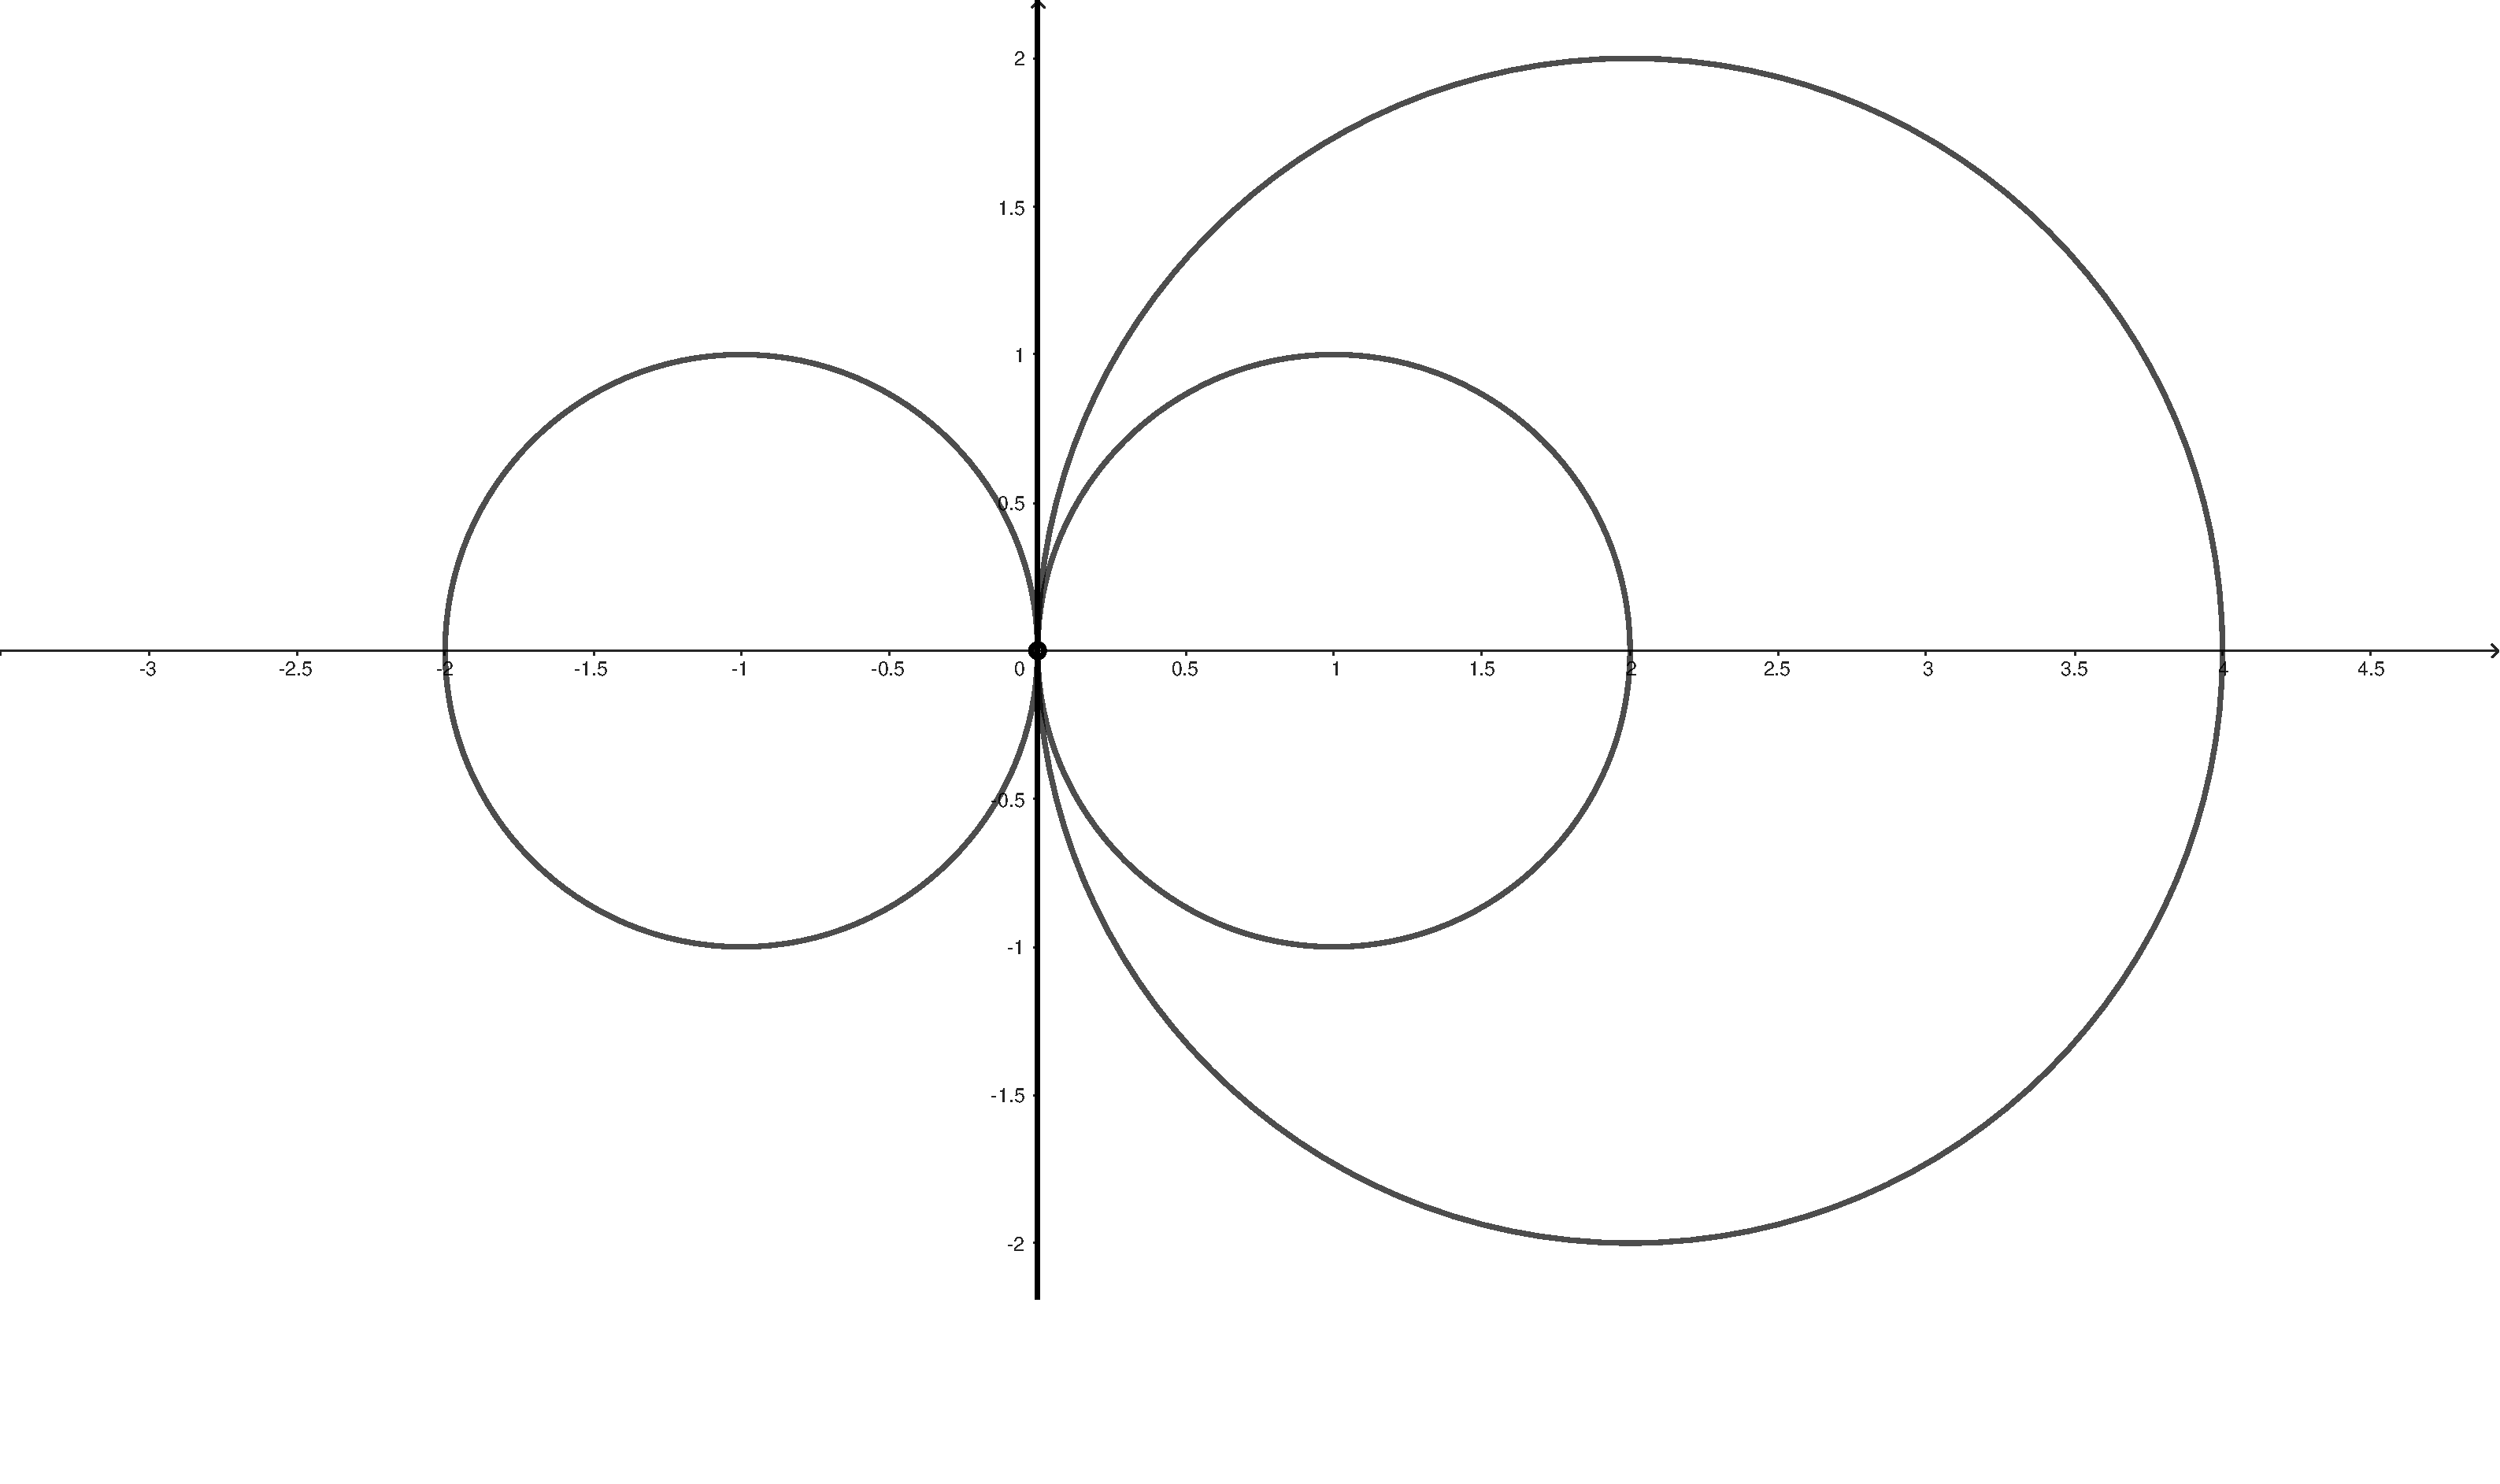
\includegraphics[width=.72\columnwidth]{figure/18.3.pdf}
\end{center}
\vskip -.3in

\subquestion{5}
\(\alpha\) 非负, \(z\neq-1\).

\(\lvert\frac{z-1}{z+1}\rvert^2=\frac{(x-1)^2+y^2}{(x+1)^2+y^2}=\alpha^2\).

若 \(\alpha=0\), 得 \(x=1, y=0\), 是点 \((1, 0)\).

若 \(\alpha=1\), 得 \(x=0\), 是虚轴.

否则, 得 \(\left(x-\frac{1+\alpha^2}{1-\alpha^2}\right)^2+y^2=\left(\frac{2\alpha}{1-\alpha^2}\right)^2\), 是以点 $(\pm1, 0)$ 为对称点的 Apollonius 圆族.\footnote{\url{https://en.wikipedia.org/wiki/Apollonian_circles}.}

\begin{center}
  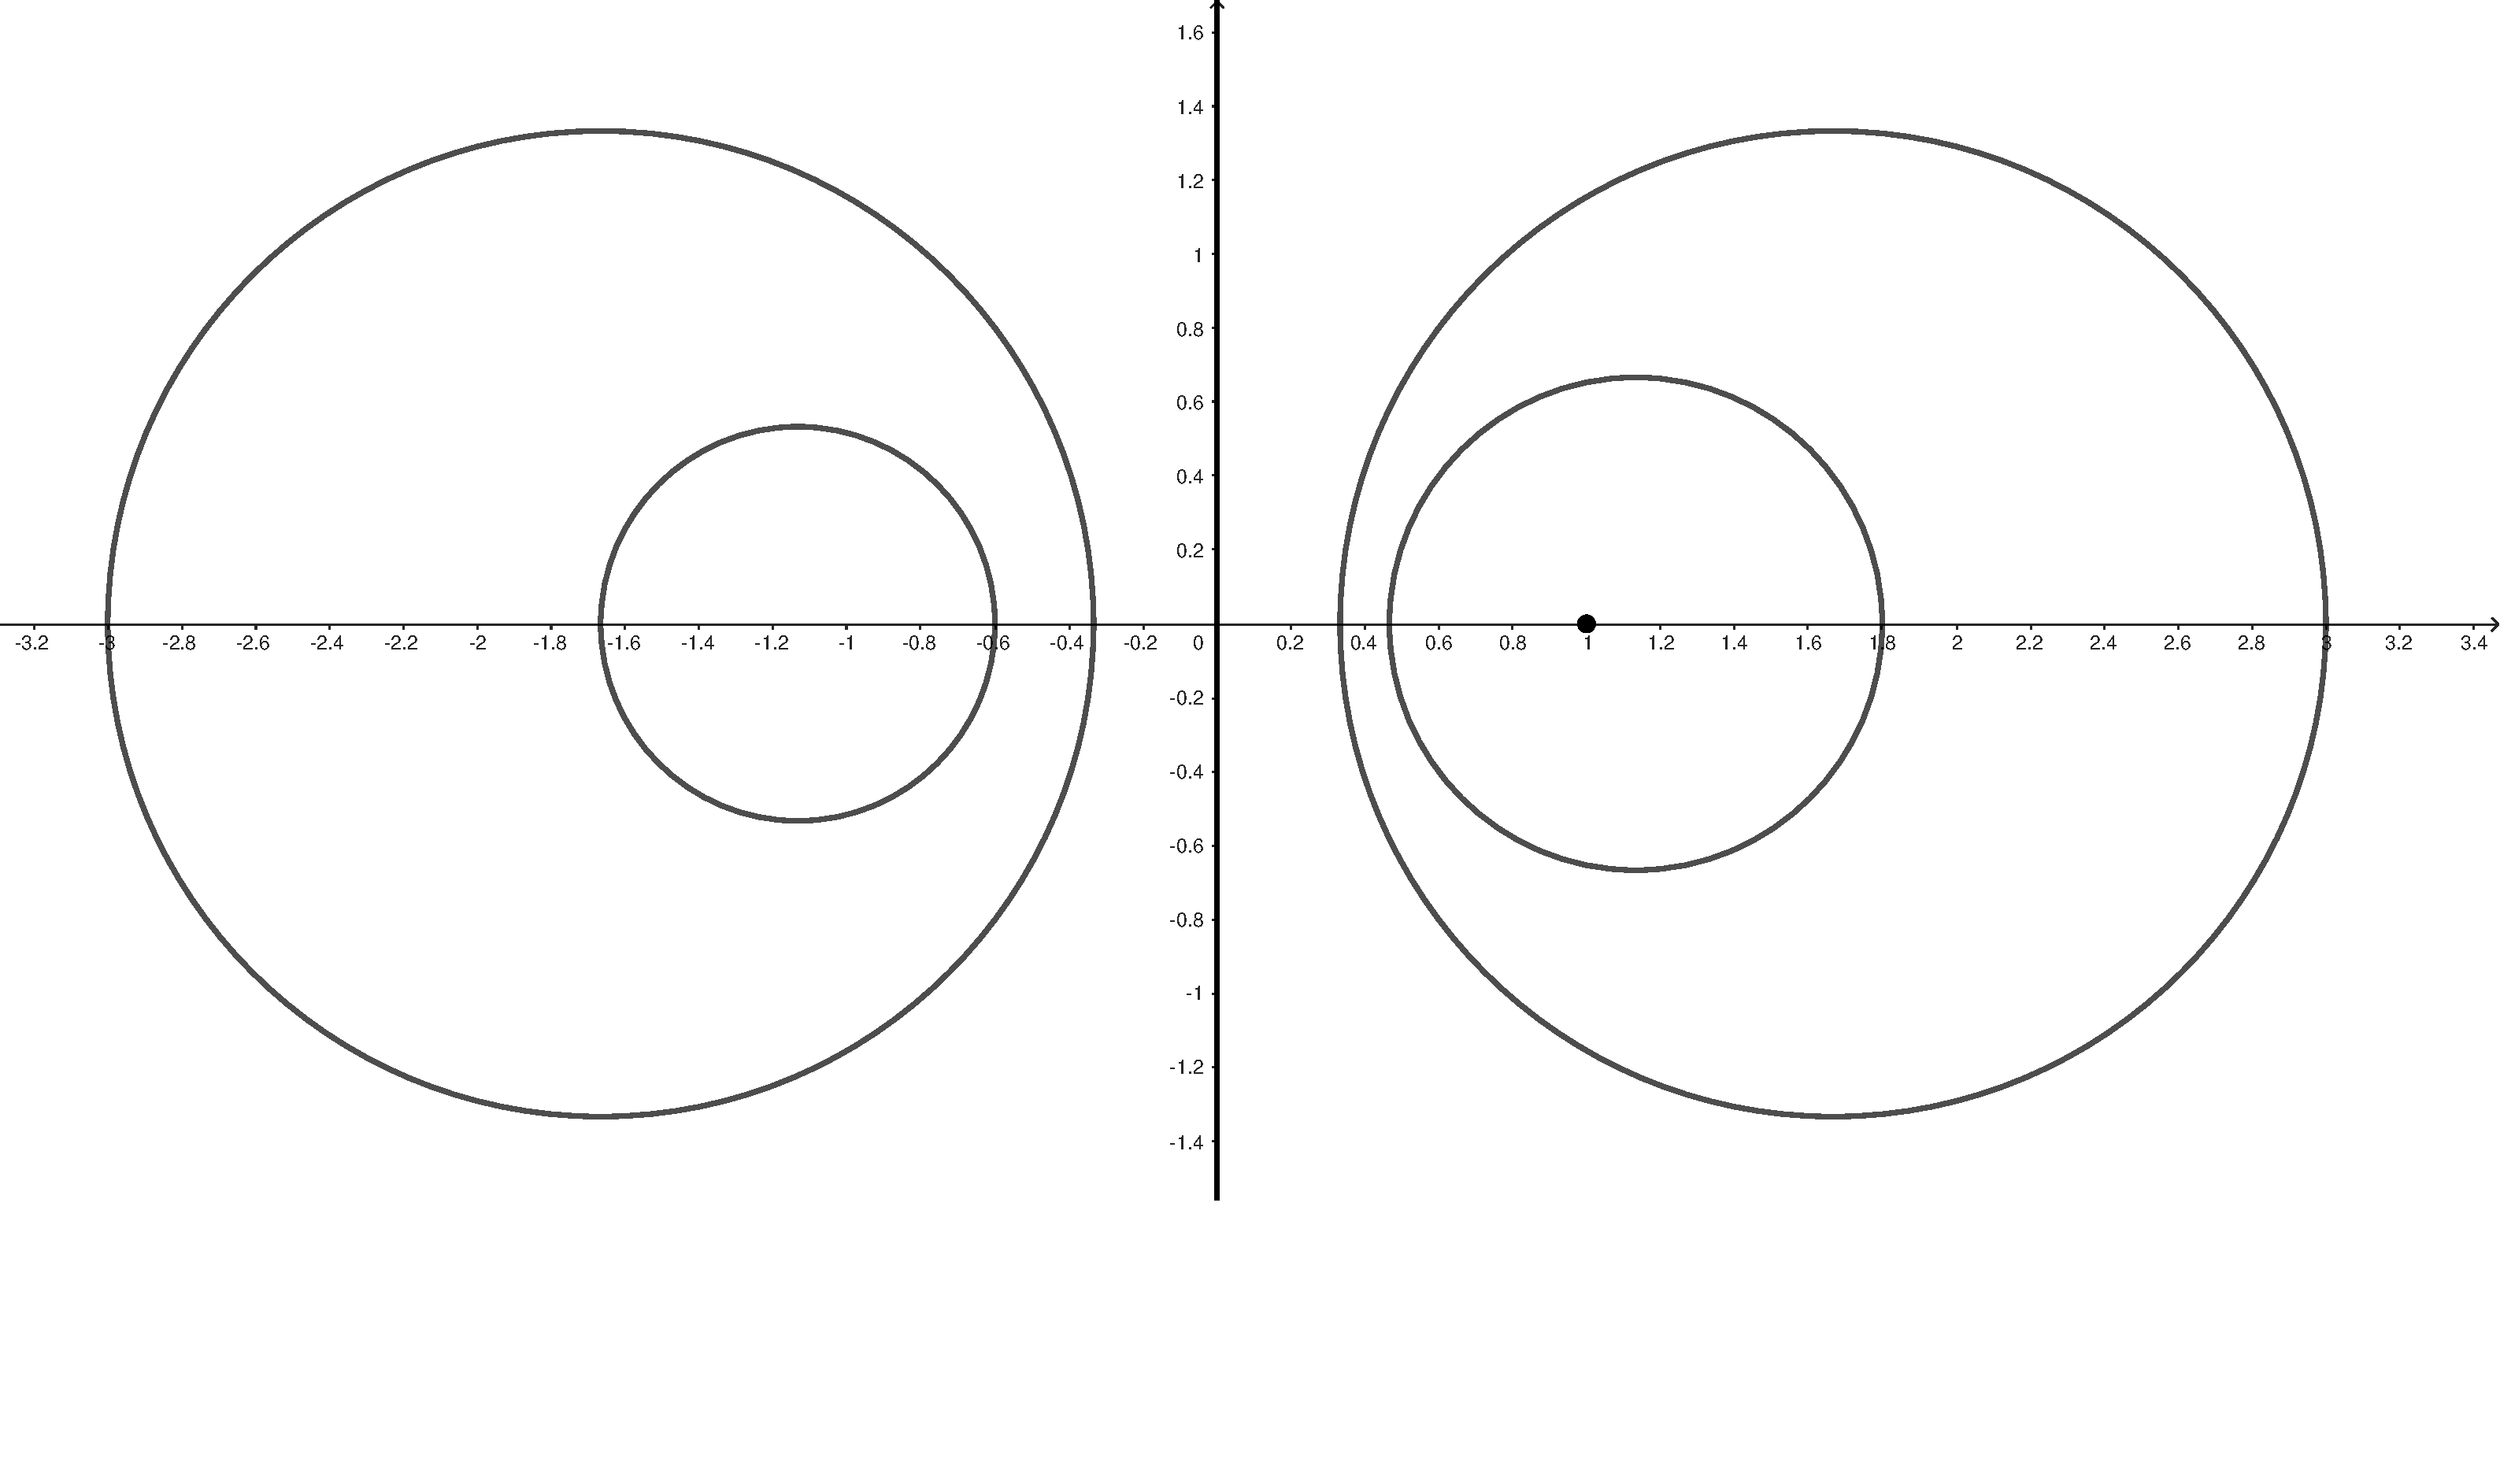
\includegraphics[width=.72\columnwidth]{figure/18.5.pdf}
\end{center}

\question{19}
\subquestion{6}
不是区域, 边界为 \(\{(x, y)\mid x=-2, \sqrt{3}\leq|y|\leq 2\sqrt{2}\}\cup\{(x, y)\mid x=\frac{3}{2}, |y|\leq\frac{\sqrt{11}}{2}\}\cup\{(x, y)\mid(x+1)^2+y^2=4, x\geq-2\}\cup\{(x, y)\mid(x+1)^2+y^2=9, -2\leq x\leq\frac{3}{2}\}\).

\begin{center}
  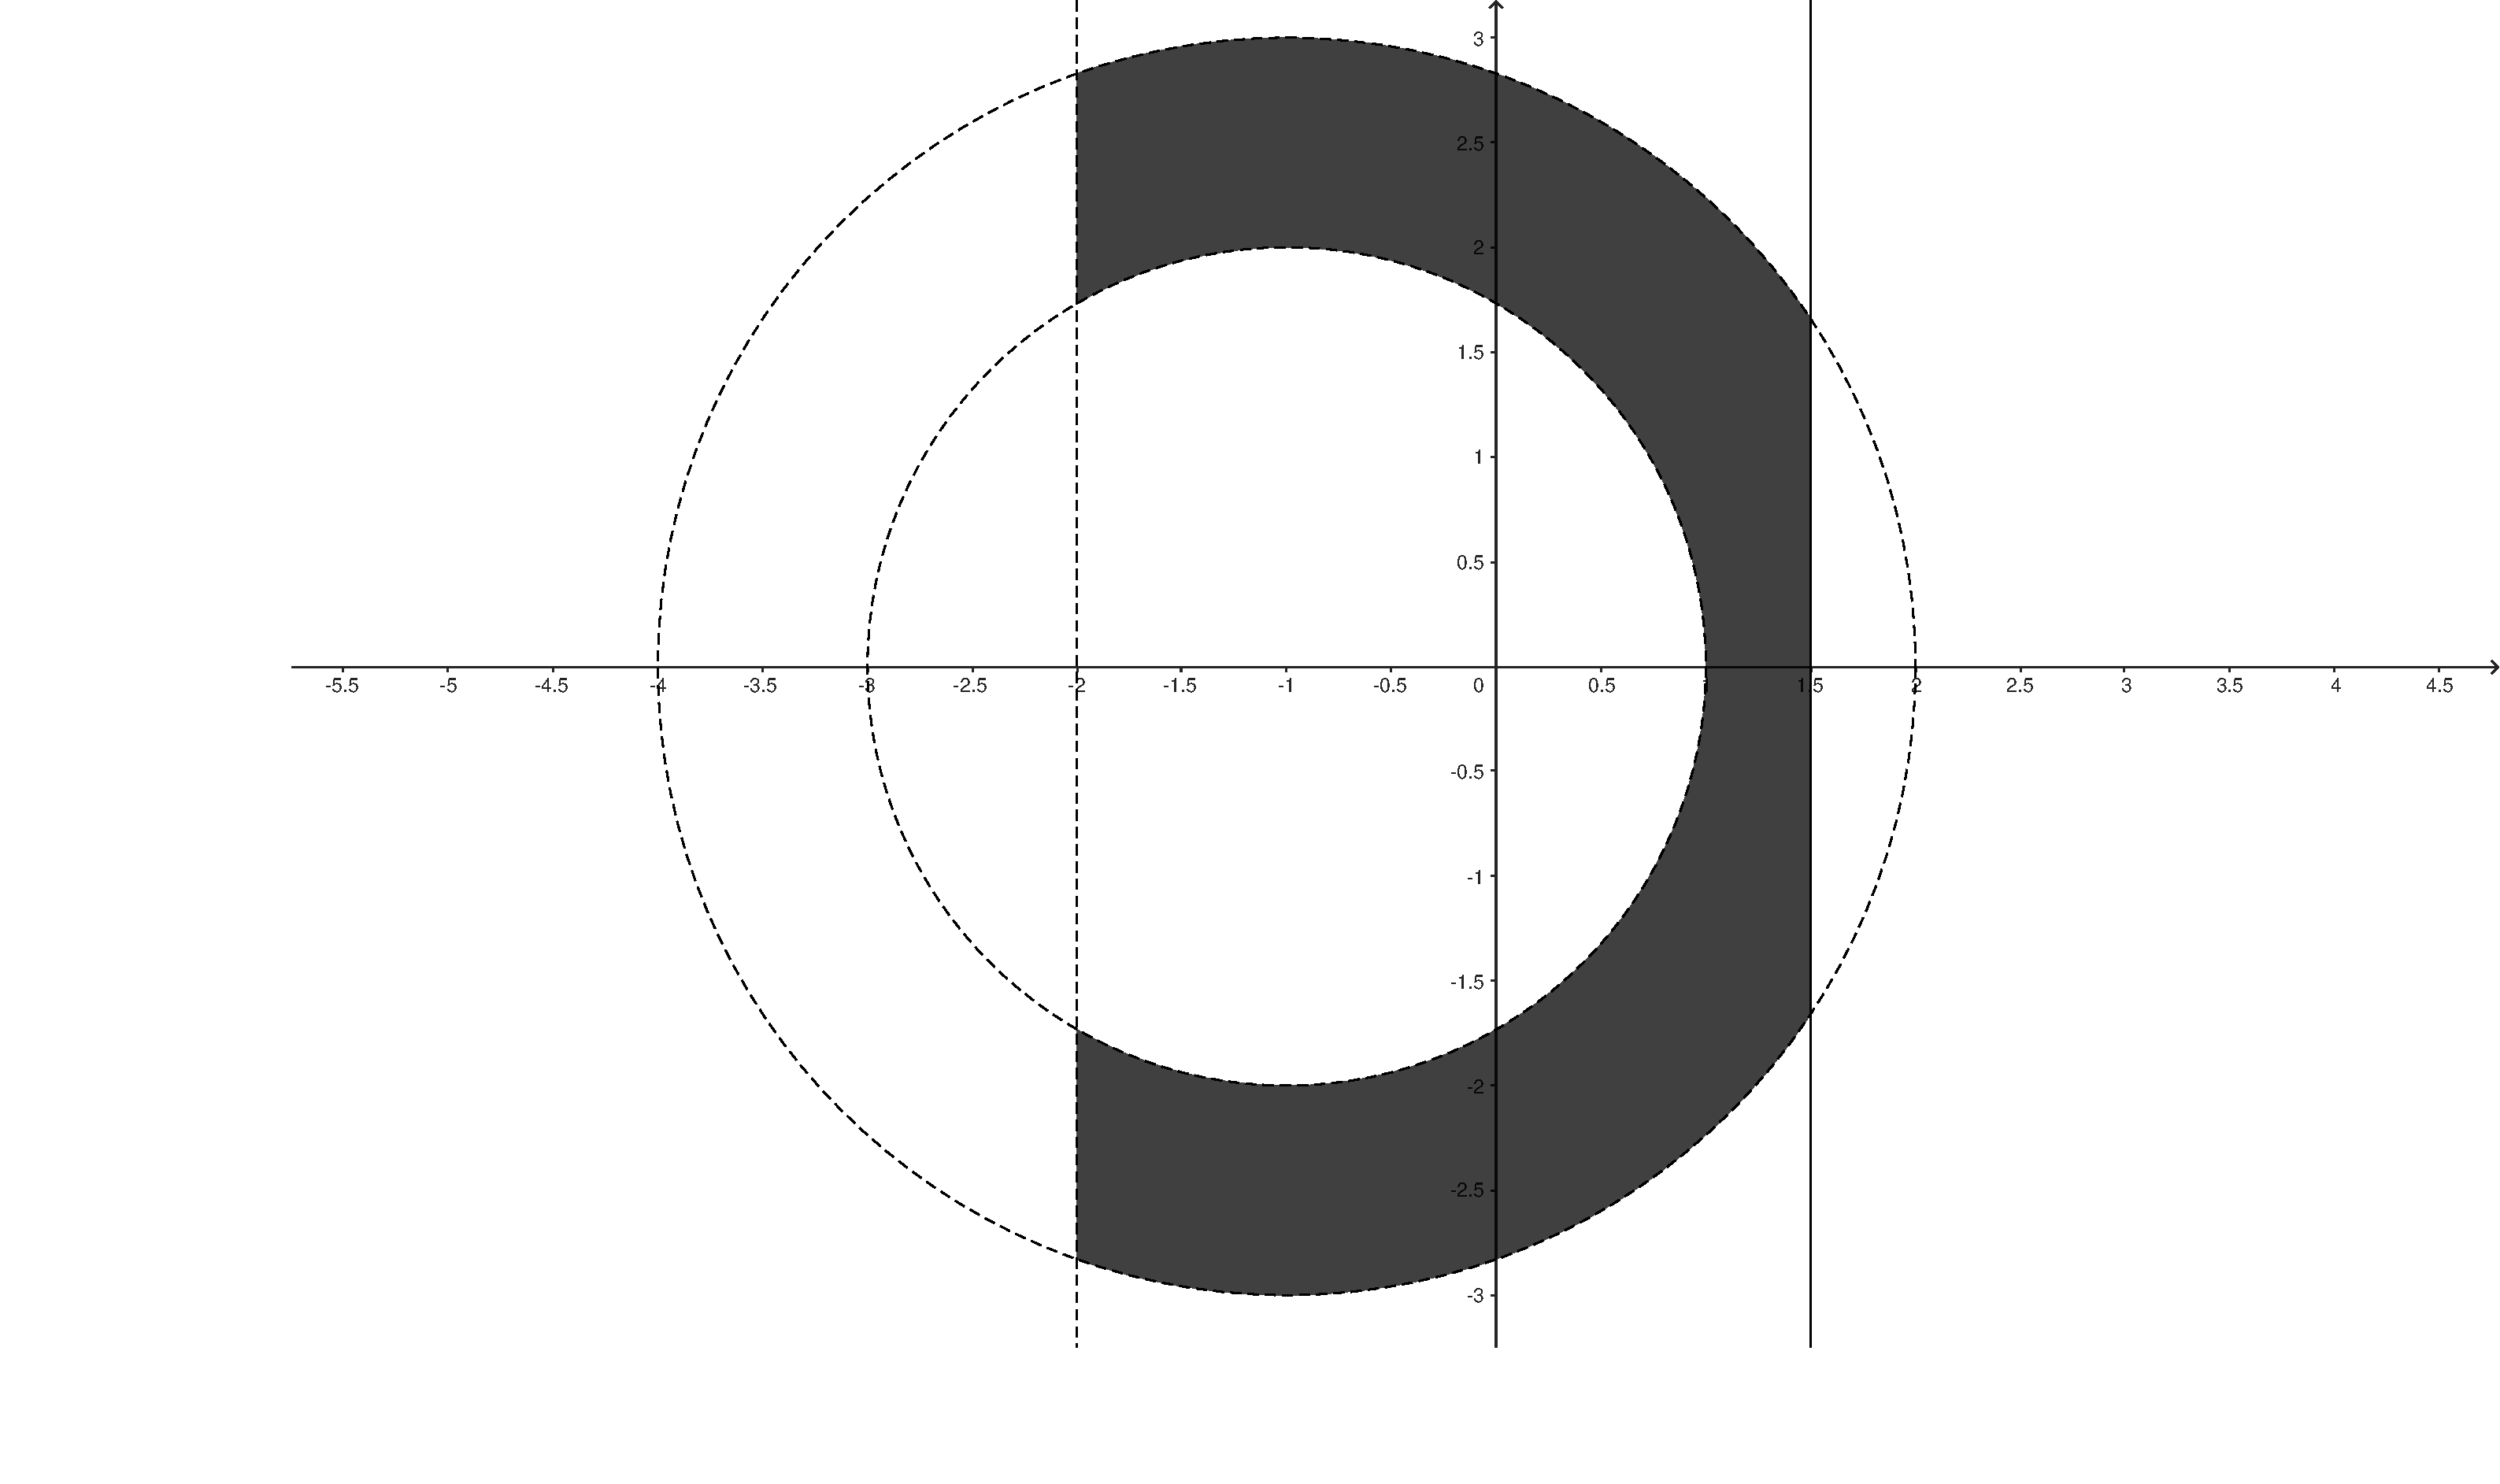
\includegraphics[width=.72\columnwidth]{figure/19.6.pdf}
\end{center}

\subquestion{10}
是区域, 边界为 \(\{(x, y)\mid x=0\)\}.
\begin{center}
  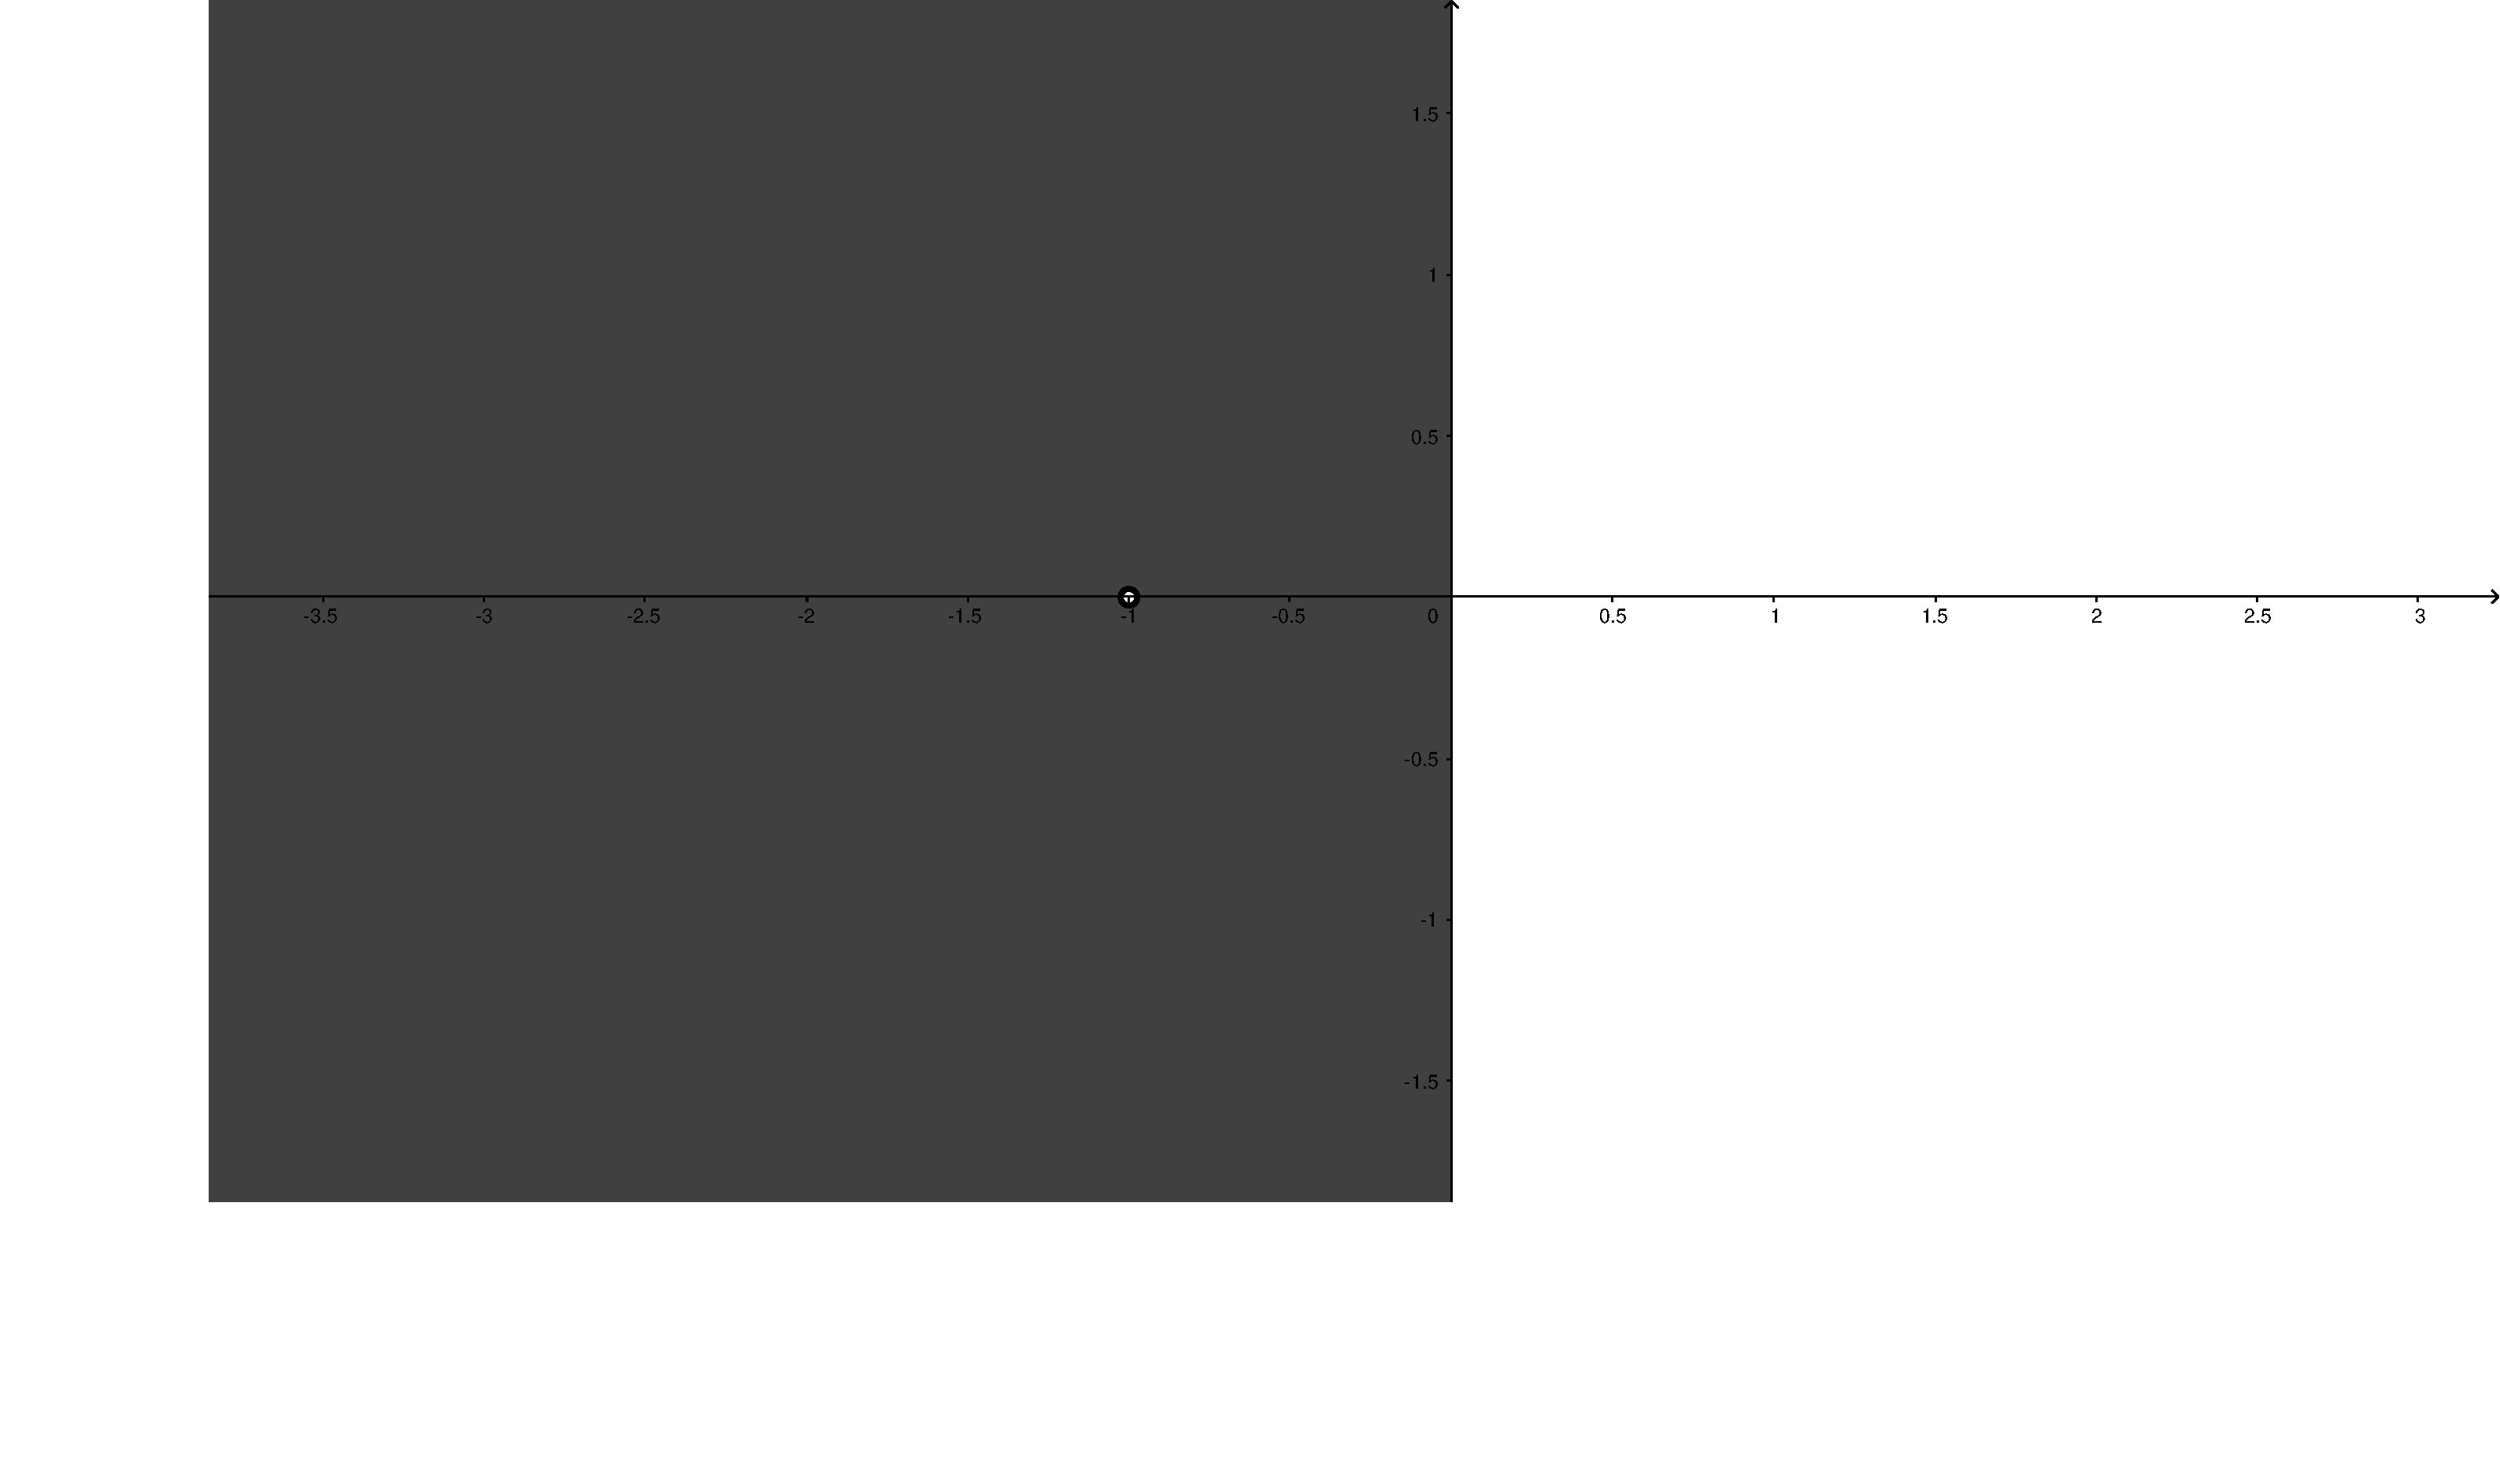
\includegraphics[width=.72\columnwidth]{figure/19.10.pdf}
\end{center}

\fbox{\parbox{\textwidth}{注释: 这题很多人错, 请自行阅读教材 1.3 节.}}

\question{21}
\subquestion{3}
设 \(z=x+iy\), 则 \(xy=1\), 是双曲线.

\question{22}
配方, 得 \((x+1)^2+y^2=2\).

设 \(z=x+iy\), 则 \(|z+1|^2=2\), 即 \(|z+1|=\sqrt{2}\).

\fbox{\parbox{\textwidth}{注释: 通法是代入 \(x=\frac{z+\overline{z}}{2}, y=\frac{z-\overline{z}}{2}\) 暴力计算.}}

\end{document}